\chapter{GroundOne Studio: a local application and a case study}
\label{ch:studio}

% Source notes: Project/docs/demo_architecture.md (§13), Project/demo/docs/progress.md, Project/docs/thesis_notes.md.

The previous chapters measure GroundOne as an isolated component. This chapter puts it to work inside a complete
application, GroundOne Studio, a RAG assistant for macOS in which document retrieval, answer generation and verification
take place in the same process, on the same 16\,GB laptop used for the experiments. The aim is twofold. On the one hand,
the application completes the argument for locality (Chapter~\ref{sec:local}): it is not enough for the verifier to be
able to run locally; it must also be shown that a usable system can be built around it without any external service. On
the other hand, it makes visible, on real answers, the properties measured in Chapter~\ref{sec:results}: the
verification of every sentence in a single forward pass, the calibrated probabilities, the comparison with a generative
LLM judge. The measurements collected in the application form a case study and are kept separate from the results of
Chapter~\ref{sec:results}: they describe the behaviour of the complete system and do not establish new records.

\section{Goals and requirements}
\label{sec:studio-goals}

The application was designed around five elements that the user must be able to see, each tied to a claim of the thesis
(Table~\ref{tab:studio-requirements}). One constraint applies to all of them: no data leaves the machine. Models,
document index, conversations and logs reside on the local disk, and the application works without a network
connection.

\begin{table}[htbp]
\centering
\caption{What the application shows and which claim of the thesis it supports.}
\label{tab:studio-requirements}
\small
\begin{tabular}{>{\raggedright\arraybackslash}p{6.2cm}>{\raggedright\arraybackslash}p{6.8cm}}
\toprule
What the user sees & Claim supported \\
\midrule
Every sentence of the answer coloured according to the GroundOne verdict, with the calibrated probabilities. & The probabilities are usable and consistent with the label shown (RQ3). \\ \addlinespace[2pt]
The comparison, on the same answer, with an LLM judge run locally: verdicts and times side by side. & Reading all the verdicts in a single forward pass, without generating text, is more accurate than an LLM judge that writes the verdicts, and faster, increasingly so as the answer grows longer (RQ2). \\ \addlinespace[2pt]
A panel with the generation and verification times and the memory in use. & Generator and verifier coexist in 16\,GB, and verification costs little compared with generation (RQ4). \\ \addlinespace[2pt]
The rewriting of the flagged sentences from the documents, verified again. & Verification is cheap enough to sit inside the generation loop. \\ \addlinespace[2pt]
For every sentence, the passage of the document that supports or contradicts it, highlighted. & Attribution to the passage can be obtained with the same model; it is an unevaluated prototype (Section~\ref{sec:concl-future}). \\
\bottomrule
\end{tabular}
\end{table}

\section{Platform choices}
\label{sec:studio-platform}

The application is written in Swift, with a SwiftUI interface, and runs the models with MLX Swift~\cite{apple2026mlxswift,
apple2026mlxswiftlm}, the Swift version of the same library used to train GroundOne. Three alternatives were considered:
a Python application around the existing package, with a web interface; a Rust application, with unofficial bindings to
MLX~\cite{oxiglade2026mlxrs} or with another runtime; a port to llama.cpp with weights converted to the GGUF format. The
first would have shown that the experiment can be served locally, but as a server and a page in the browser, not as an
installable application. The last two would have required demonstrating numerical equivalence with the results anew,
and in the case of llama.cpp recalibrating the model after a new quantisation. MLX Swift, by contrast, loads the same
weights and the same adapter and relies on the same MLX backend: if a conformance test confirms it
(Section~\ref{sec:studio-port}), the numbers of the thesis also hold for the application, without retraining or
recalibrating anything. The price is portability: the interface is tied to Apple platforms, and compiling the MLX
shaders requires Xcode.

\section{Architecture}
\label{sec:studio-architecture}

The application is divided into three layers (Figure~\ref{fig:studio-architecture}). The first is the interface. The
second is a core that does not depend on the engines: it manages the session (answer, verification, rewriting), applies
the policy and saves conversations and logs. The core knows only five abstract interfaces, called \emph{ports}:
retriever, generator, verifier, LLM judge and attributor. The third layer contains the engines that implement them. Thanks
to this separation the core was tested with fake, deterministic engines, just as the Python package is tested with a
fake backend, and a different engine, for example a generator on llama.cpp, could replace the current one without
touching the rest.

\begin{figure}[htbp]
\centering
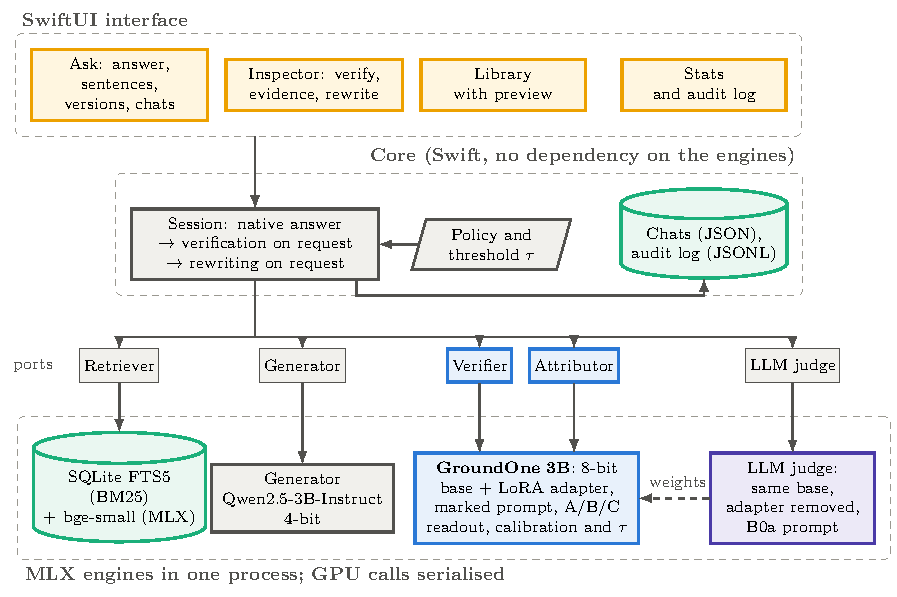
\includegraphics[width=\textwidth]{images/diagrams/studio_architecture_tikz.pdf}
\caption{Architecture of GroundOne Studio. The core knows only the ports; the engines, all in the same process, are the
retriever, the generator, GroundOne (verifier and, passage by passage, attributor) and the LLM judge, which uses the same
weights as GroundOne with the adapter removed. The components in which GroundOne is involved are shown in blue.}
\label{fig:studio-architecture}
\end{figure}

There are four engines. The generator is Qwen2.5-3B-Instruct quantised to 4 bits, the same one used in the
co-residence measurement of Section~\ref{sec:results-locality}. The verifier is GroundOne 3B, that is, the 8-bit base
with the LoRA adapter, the marker prompt, the readout of the letters A, B and C and the calibration fitted on the dev
set. It is the default model because it is the most accurate, and in the application verification happens only on request, in about two seconds for a typical answer read from scratch and in about half a second once the sources have been read ahead (Section~\ref{sec:studio-flow}); a selector allows switching to the faster 0.5B. The LLM judge used
for the comparison is the same base model as GroundOne with the adapter removed at runtime and the prompt of the terse
LLM judge B0a (Section~\ref{sec:setup-baselines}): it is exactly the LLM judge measured in the thesis, it takes no additional
memory and it does not leave the machine. The retriever, finally, combines a full-text index and a small embedding model
(Section~\ref{sec:studio-library}).

All calls to the models go through the model containers of MLX Swift, which serialise access to them, and are executed
one at a time on the GPU, as happens with the single worker thread of the Python service
(Section~\ref{sec:method-software}). Generation and verification therefore do not compete for resources, and the measured times are not confounded by concurrent executions. The read-ahead of the sources, which starts in the background when an answer is complete, follows the same rule: a verification, a comparison with the LLM judge or a new answer requested while it is running waits for it to finish. With the three models loaded, the memory allocated by MLX is
about 5.3\,GB and reaches a peak of 6.2\,GB during one question and of 6.9\,GB after a session of twelve questions, when the KV cache also keeps the sources of the earlier ones. The first value is in line with the co-residence measurement of
Table~\ref{tab:results-coresidence}, which did not include the retriever. The embedding model therefore adds little: it
takes about 130\,MB on disk.

\section{Porting GroundOne to Swift}
\label{sec:studio-port}

Four parts of GroundOne were rewritten in Swift; the rest, namely weights, adapter and calibration, is loaded as it is.
The first is prompt construction. As in training, header, numbered sentences, markers and line breaks are tokenised
separately and then concatenated, because tokenising the joined string would produce different identifiers at the
boundaries between the pieces. The tokeniser is that of swift-transformers~\cite{hf2026swifttransformers}. The second is
the readout: the model computes the hidden states of the whole sequence, but the output head is applied only at the
marker positions, and at each of them only the logits of the three letters are read. The third is calibration:
temperature, bias and threshold $\tau$ are read from the same file produced in Python. The fourth is sentence
segmentation: PySBD does not exist for Swift, and the segmentation rule of Section~\ref{sec:data-construction} was
reproduced with the sentence tokeniser of the operating system~\cite{apple2026nltokenizer}, adding the same rules for
lists and for checkable content.

\paragraph{Conformance test.} Before the interface was built, the port was compared with Python on 200 answers of T1,
stratified by number of sentences like the subset used for latency, for a total of 1{,}747 markers. For every answer,
Python exports the token identifiers, the marker positions, the logits, the calibrated probabilities and the labels;
Swift must reproduce them (Table~\ref{tab:studio-conformance}). The token identifiers and the marker positions coincide
in all 200 answers with both models. With the 3B, the default model of the application, the maximum difference between
the calibrated probabilities is 0.005 and all the labels coincide: for the same input, the results of the thesis
therefore also hold for the verifier of the application. With the 0.5B, three sentences out of 1{,}747 exceed a
difference of 0.01, with a maximum of 0.031, and the labels coincide in 99.71\,\% of the cases; every disagreement
concerns a sentence whose probability of support falls within 0.01 of the threshold. A plausible but unverified cause is
a different order of summation in reduced precision, which weighs more heavily on the small model. The same test compares in Swift the cached path, which reuses the sources or the beginning of an answer already verified after a one-token change, with the pass without cache: the probabilities differ by at most 0.007 with the 3B and 0.019 with the 0.5B, the same order of magnitude observed in Python (Section~\ref{sec:results-latency-split}).

\begin{table}[htbp]
\centering
\caption{Conformance test between the Swift and the Python implementations on 200 answers of T1 (1{,}747 markers). The
logits are computed in Swift on the same token identifiers produced by Python.}
\label{tab:studio-conformance}
\small
\begin{tabular}{>{\raggedright\arraybackslash}p{6.6cm}cc}
\toprule
Check & GroundOne 3B & GroundOne 0.5B \\
\midrule
Identical token identifiers and marker positions & 200/200 & 200/200 \\
Maximum difference between the logits & 0.070 & 0.172 \\
Maximum difference between the calibrated probabilities & 0.005 & 0.031 \\
Sentences with a probability difference below 0.01 & 100\,\% & 99.83\,\% \\
Identical served labels & 100\,\% & 99.71\,\% \\
Maximum difference between the probabilities with and without the cache & 0.007 & 0.019 \\
\bottomrule
\end{tabular}
\end{table}

Speed is also almost the same. On the same 200 answers, verification takes on average 2.13 seconds in Swift against
2.04 in Python with the 3B, about 4\,\% more, and 0.34 against 0.33 seconds with the 0.5B; these are means, whereas
Chapter~\ref{sec:results} reports medians. Segmentation, finally, produces the same sentences as PySBD in 98.4\,\% of the
2{,}647 answers of T1. The remaining differences mostly concern abbreviated titles and quotations that span several
sentences. Without three additional rules, which do not split the sentence after initials and common abbreviations or
before a lower-case word, and which attach list bullets to the following sentence, the agreement would fall to
95.2\,\%.

\section{Library and document retrieval}
\label{sec:studio-library}

The library of the application consists of the sources of T1: the 147 CNN and Daily Mail news articles of the
summarisation task and the 450 MS MARCO web passages of question answering, linked to the 150 real questions they come
from. The structured Yelp records, in JSON format, are excluded, because they are not documents to converse with. The
documents thus belong to the domain in which GroundOne was trained and calibrated, and the probabilities shown to the
user should largely retain their meaning. This was not measured: generator, prompt and a context made of several
passages differ from those of RAGTruth in any case.

Every document is split into passages of about 140 words, aligned with sentence boundaries, which keep the source file
and the position in the text. Retrieval is hybrid. A full-text index in SQLite~\cite{sqlite2026fts5} ranks the passages
with BM25\footnote{BM25 is a classic scoring function of information retrieval: it rewards passages that contain the
terms of the query, giving more weight to terms that are rare in the collection and damping the effect of repetitions
and of passage length~\cite{robertson2009bm25}.}, while a small embedding model, bge-small-en-v1.5~\cite{xiao2024cpack},
also run with MLX, ranks them by semantic similarity. The two rankings are merged with reciprocal rank
fusion\footnote{\emph{Reciprocal rank fusion} assigns to every passage the sum, over the rankings to be combined, of
$1/(60 + r)$, where $r$ is the position of the passage in each ranking: a passage placed well in both outranks one that
appears at the top of only one~\cite{cormack2009rrf}.}, and every document can contribute at most three passages, so
that a comparison question reaches different sources. The six retrieved passages, preceded by the question, form the
document that GroundOne reads, in the same form as the question answering of RAGTruth.

On the 150 real MS MARCO questions, hybrid retrieval returns all the original passages of the question among the six
passages, with BM25 alone as with fusion. The result is, however, optimistic by construction: in the library every
passage is preceded by its own question, used as a title, and the question asked is identical. The measurement confirms
that the index works, not that retrieval is robust to freely formulated questions.

\section{Using the application}
\label{sec:studio-flow}

\begin{figure}[htbp]
\centering
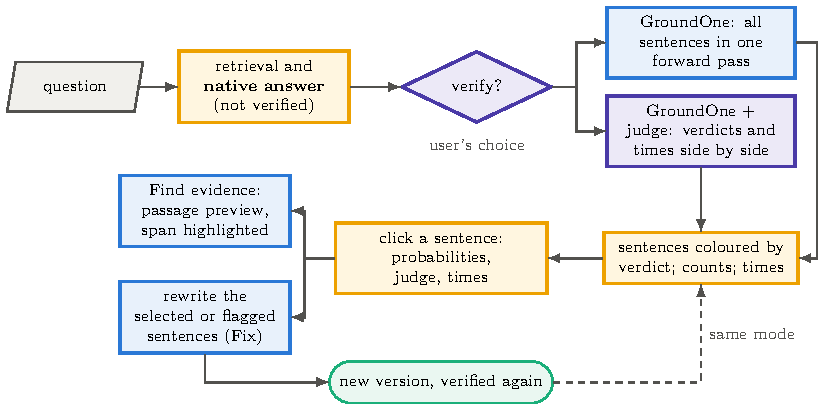
\includegraphics[width=\textwidth]{images/diagrams/studio_flow_tikz.pdf}
\caption{The usage flow. The answer appears as the generator wrote it; verification, with GroundOne or with GroundOne
and the LLM judge, and rewriting happen only on request, and every rewriting produces a new version that is verified again
in the same mode.}
\label{fig:studio-flow}
\end{figure}

The usage flow is summarised in Figure~\ref{fig:studio-flow}. The user asks a question, or picks one of the examples
offered on the start screen. The generator receives the retrieved passages and writes an answer of several paragraphs,
which appears exactly as it was generated, without any intervention (Figure~\ref{fig:studio-native}). Only at this point
does the user decide whether to verify it, and how: with GroundOne alone, or with GroundOne and the LLM judge, to
compare verdicts and times. The separation is deliberate: by showing the native answer first, the effect of verification
remains visible, instead of delivering an already filtered answer straight away. The separation also has a cost advantage. The sources are known before the answer, so, as soon as the generator has finished, GroundOne reads the instructions and the sources into its KV cache in the background while the user reads the answer, and the verification, if requested, reads only the answer. On the 200 answers of the latency measurement, with the 3B the first verification drops at the median from 2.11 to 0.59 seconds (3.6 times), while the read-ahead, 1.41 seconds, uses the GPU when it would otherwise be idle; with the 0.5B the verification drops from 0.35 to 0.10 seconds. If the user asks for the verification before the read-ahead has finished, the verification waits for it instead of repeating it, and costs as much as without read-ahead (2.11 seconds at the median with the 3B). The Python service offers the same mechanism through a dedicated call (\texttt{/v1/prefetch}).

\begin{figure}[htbp]
\centering
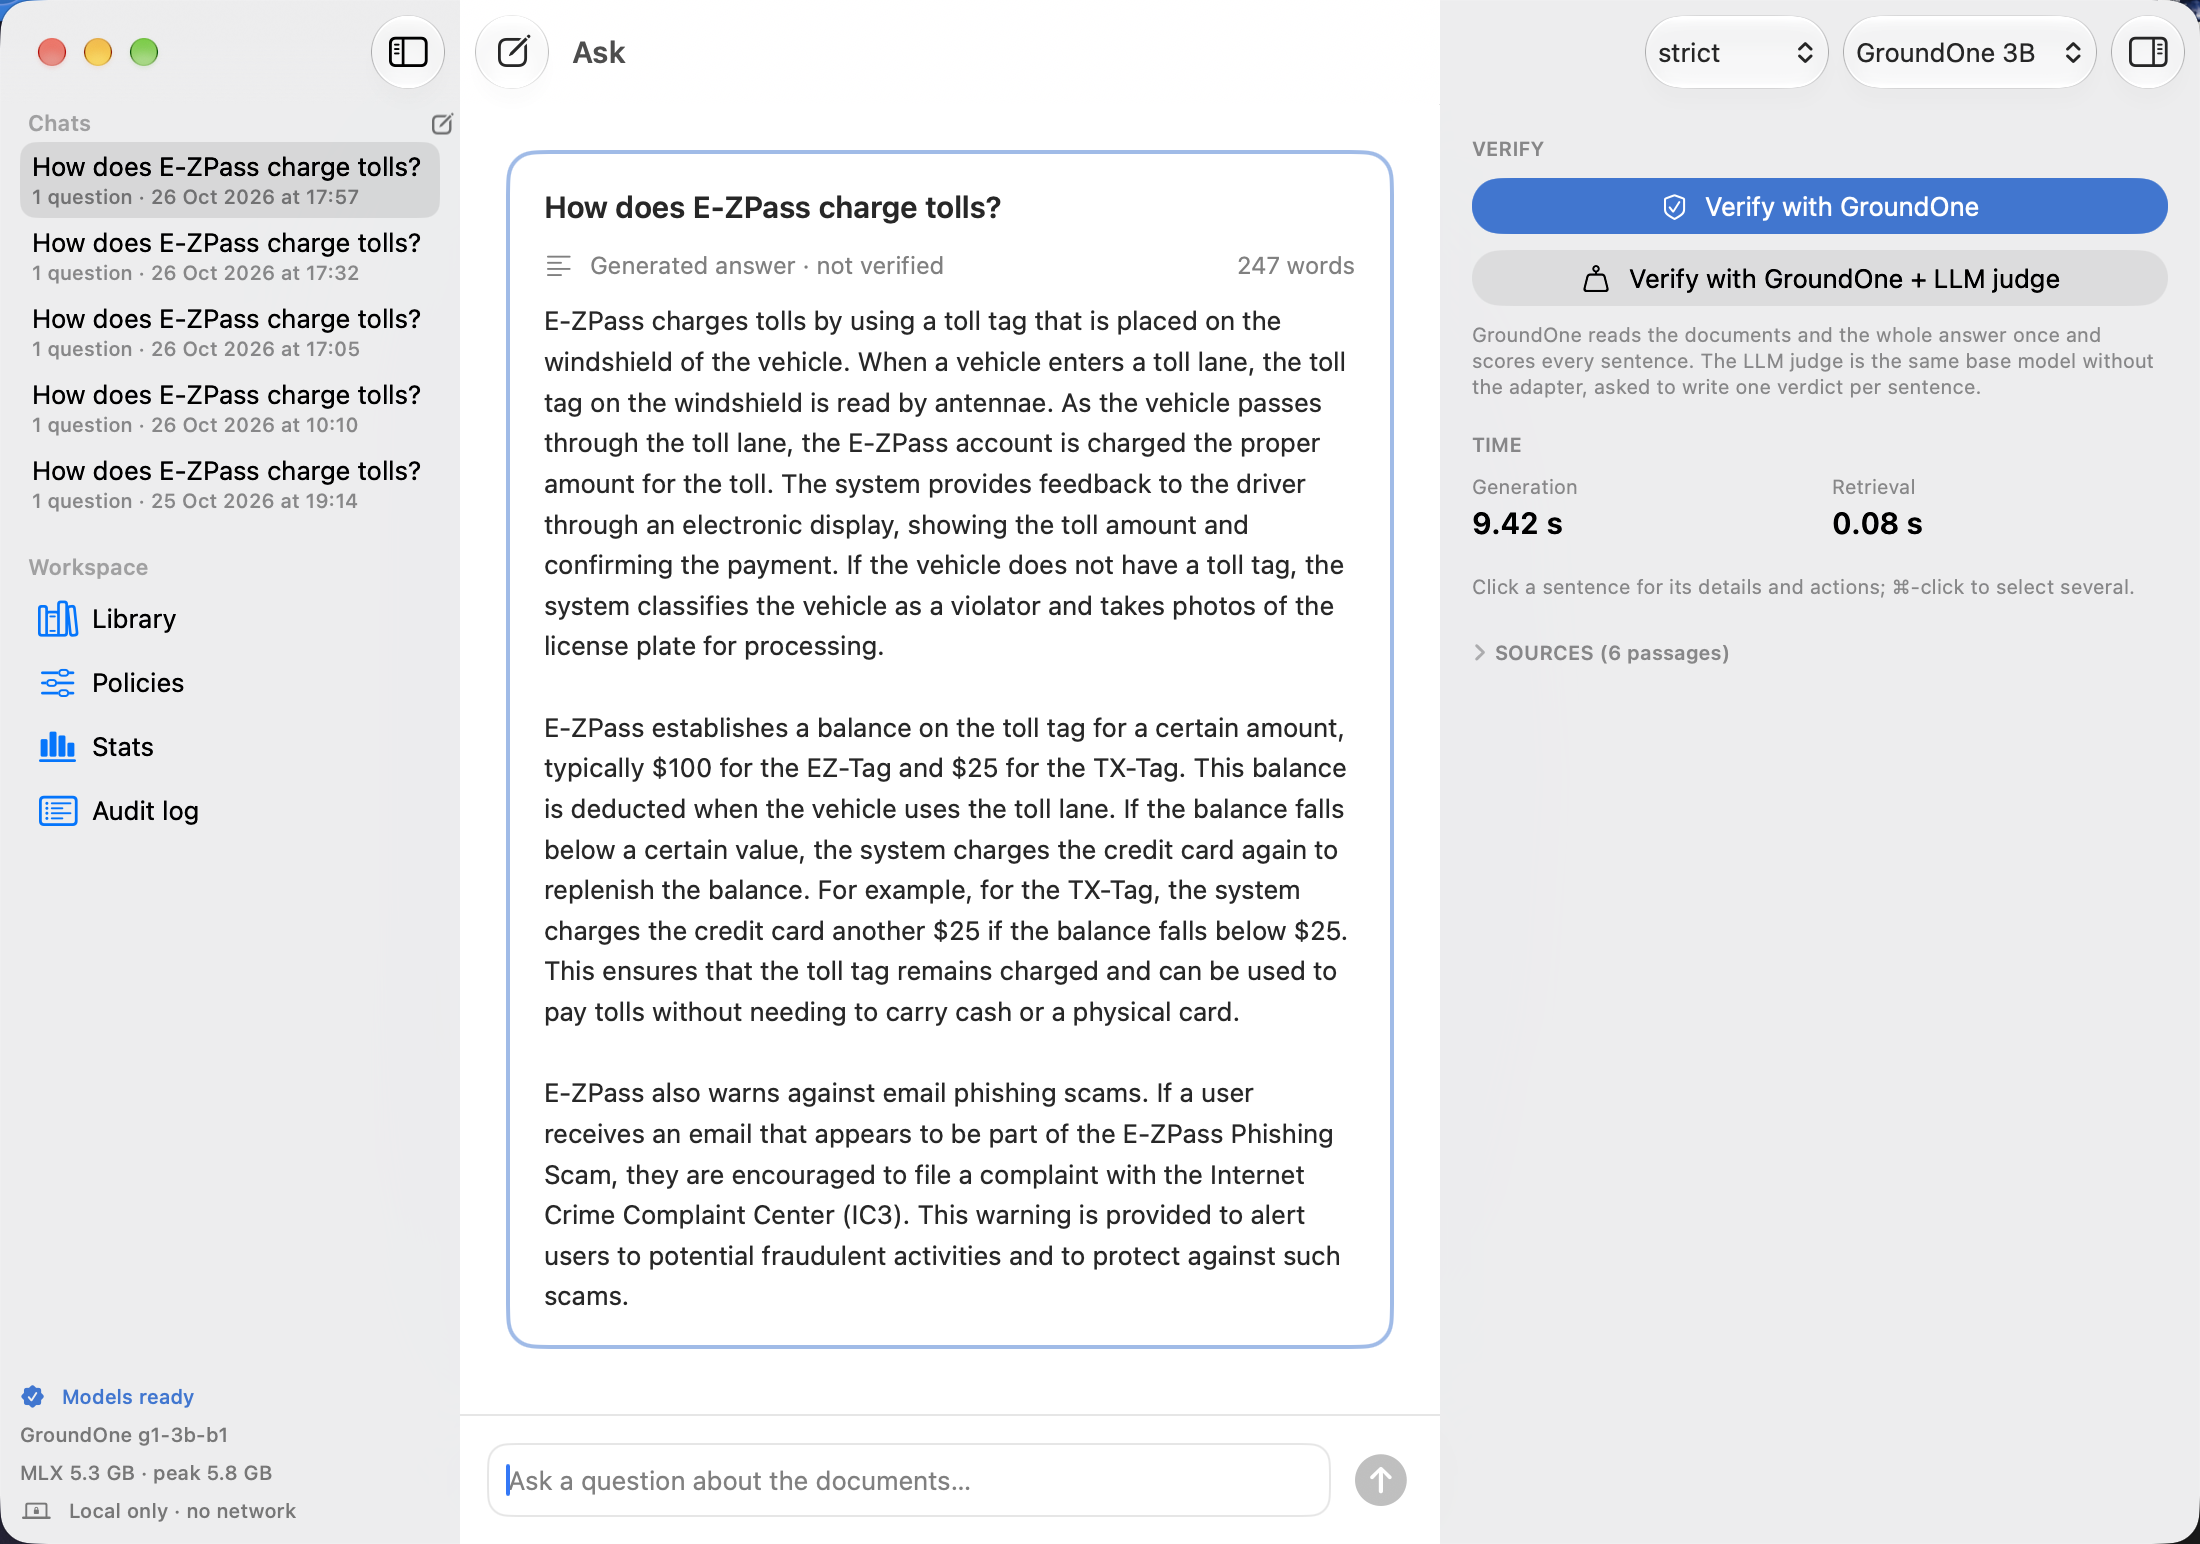
\includegraphics[width=\textwidth]{images/studio/41-native.png}
\caption{The native answer of the generator to the question ``How does E-ZPass charge tolls?'', before any
verification. The two verification modes are on the right.}
\label{fig:studio-native}
\end{figure}

GroundOne verification, in both modes, reads the whole answer in a single forward pass: all the sentences receive their
verdict together, and an answer with many sentences does not require more passes. After verification the sentences are
coloured: light green for supported sentences, red for contradicted ones, orange for those not mentioned by the
document; sentences without checkable content remain grey (Figure~\ref{fig:studio-verified}). The side panel reports the
counts, the threshold $\tau$, the times of generation, of verification and, if requested, of the LLM judge, and the
sentences on which GroundOne and the LLM judge disagree.

\begin{figure}[htbp]
\centering
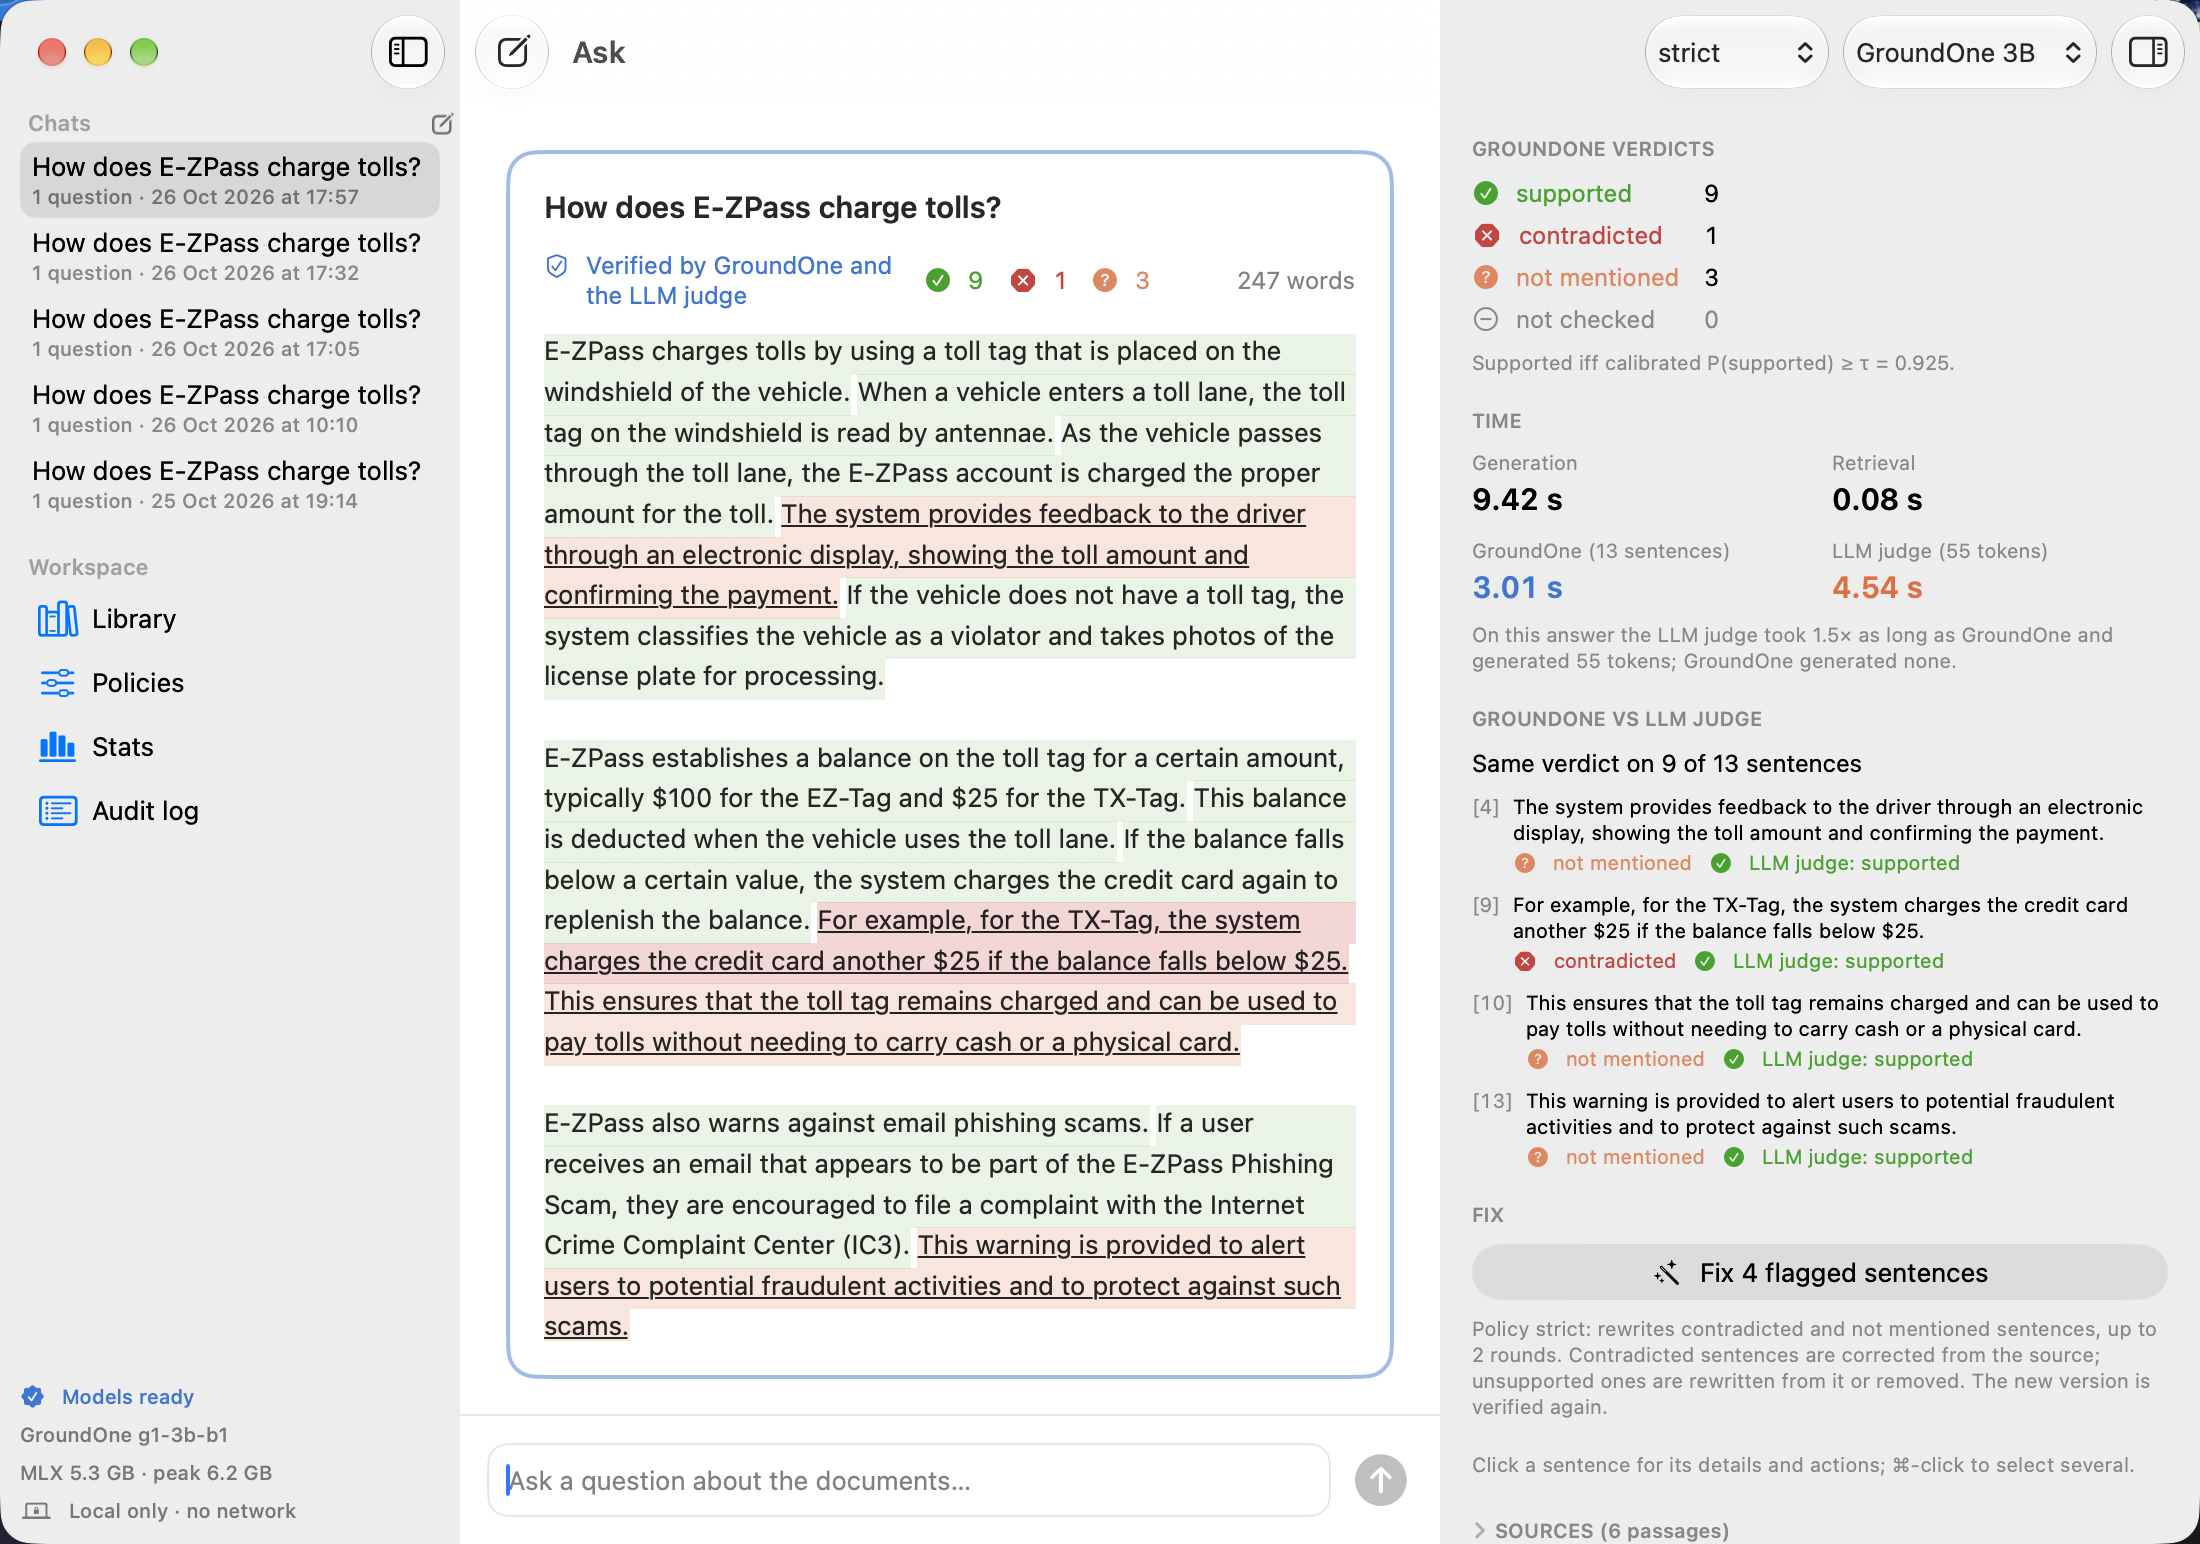
\includegraphics[width=\textwidth]{images/studio/42-verified.png}
\caption{The same answer after verification with GroundOne and the LLM judge. The sentences are coloured according to the
GroundOne verdict; the panel reports counts, times and disagreements with the LLM judge.}
\label{fig:studio-verified}
\end{figure}

Every sentence can be selected. A click shows, in the panel, the three calibrated probabilities, the verdict of the
LLM judge and the times; with the Command key several sentences can be selected (Figure~\ref{fig:studio-sentence}). From
here the user can request the supporting evidence, or the rewriting of the selected sentences. When nothing is selected,
a button rewrites all the flagged sentences according to the chosen policy. Every rewriting produces a new version of
the answer, verified again in the same mode, and a selector allows the versions to be compared.

\begin{figure}[htbp]
\centering
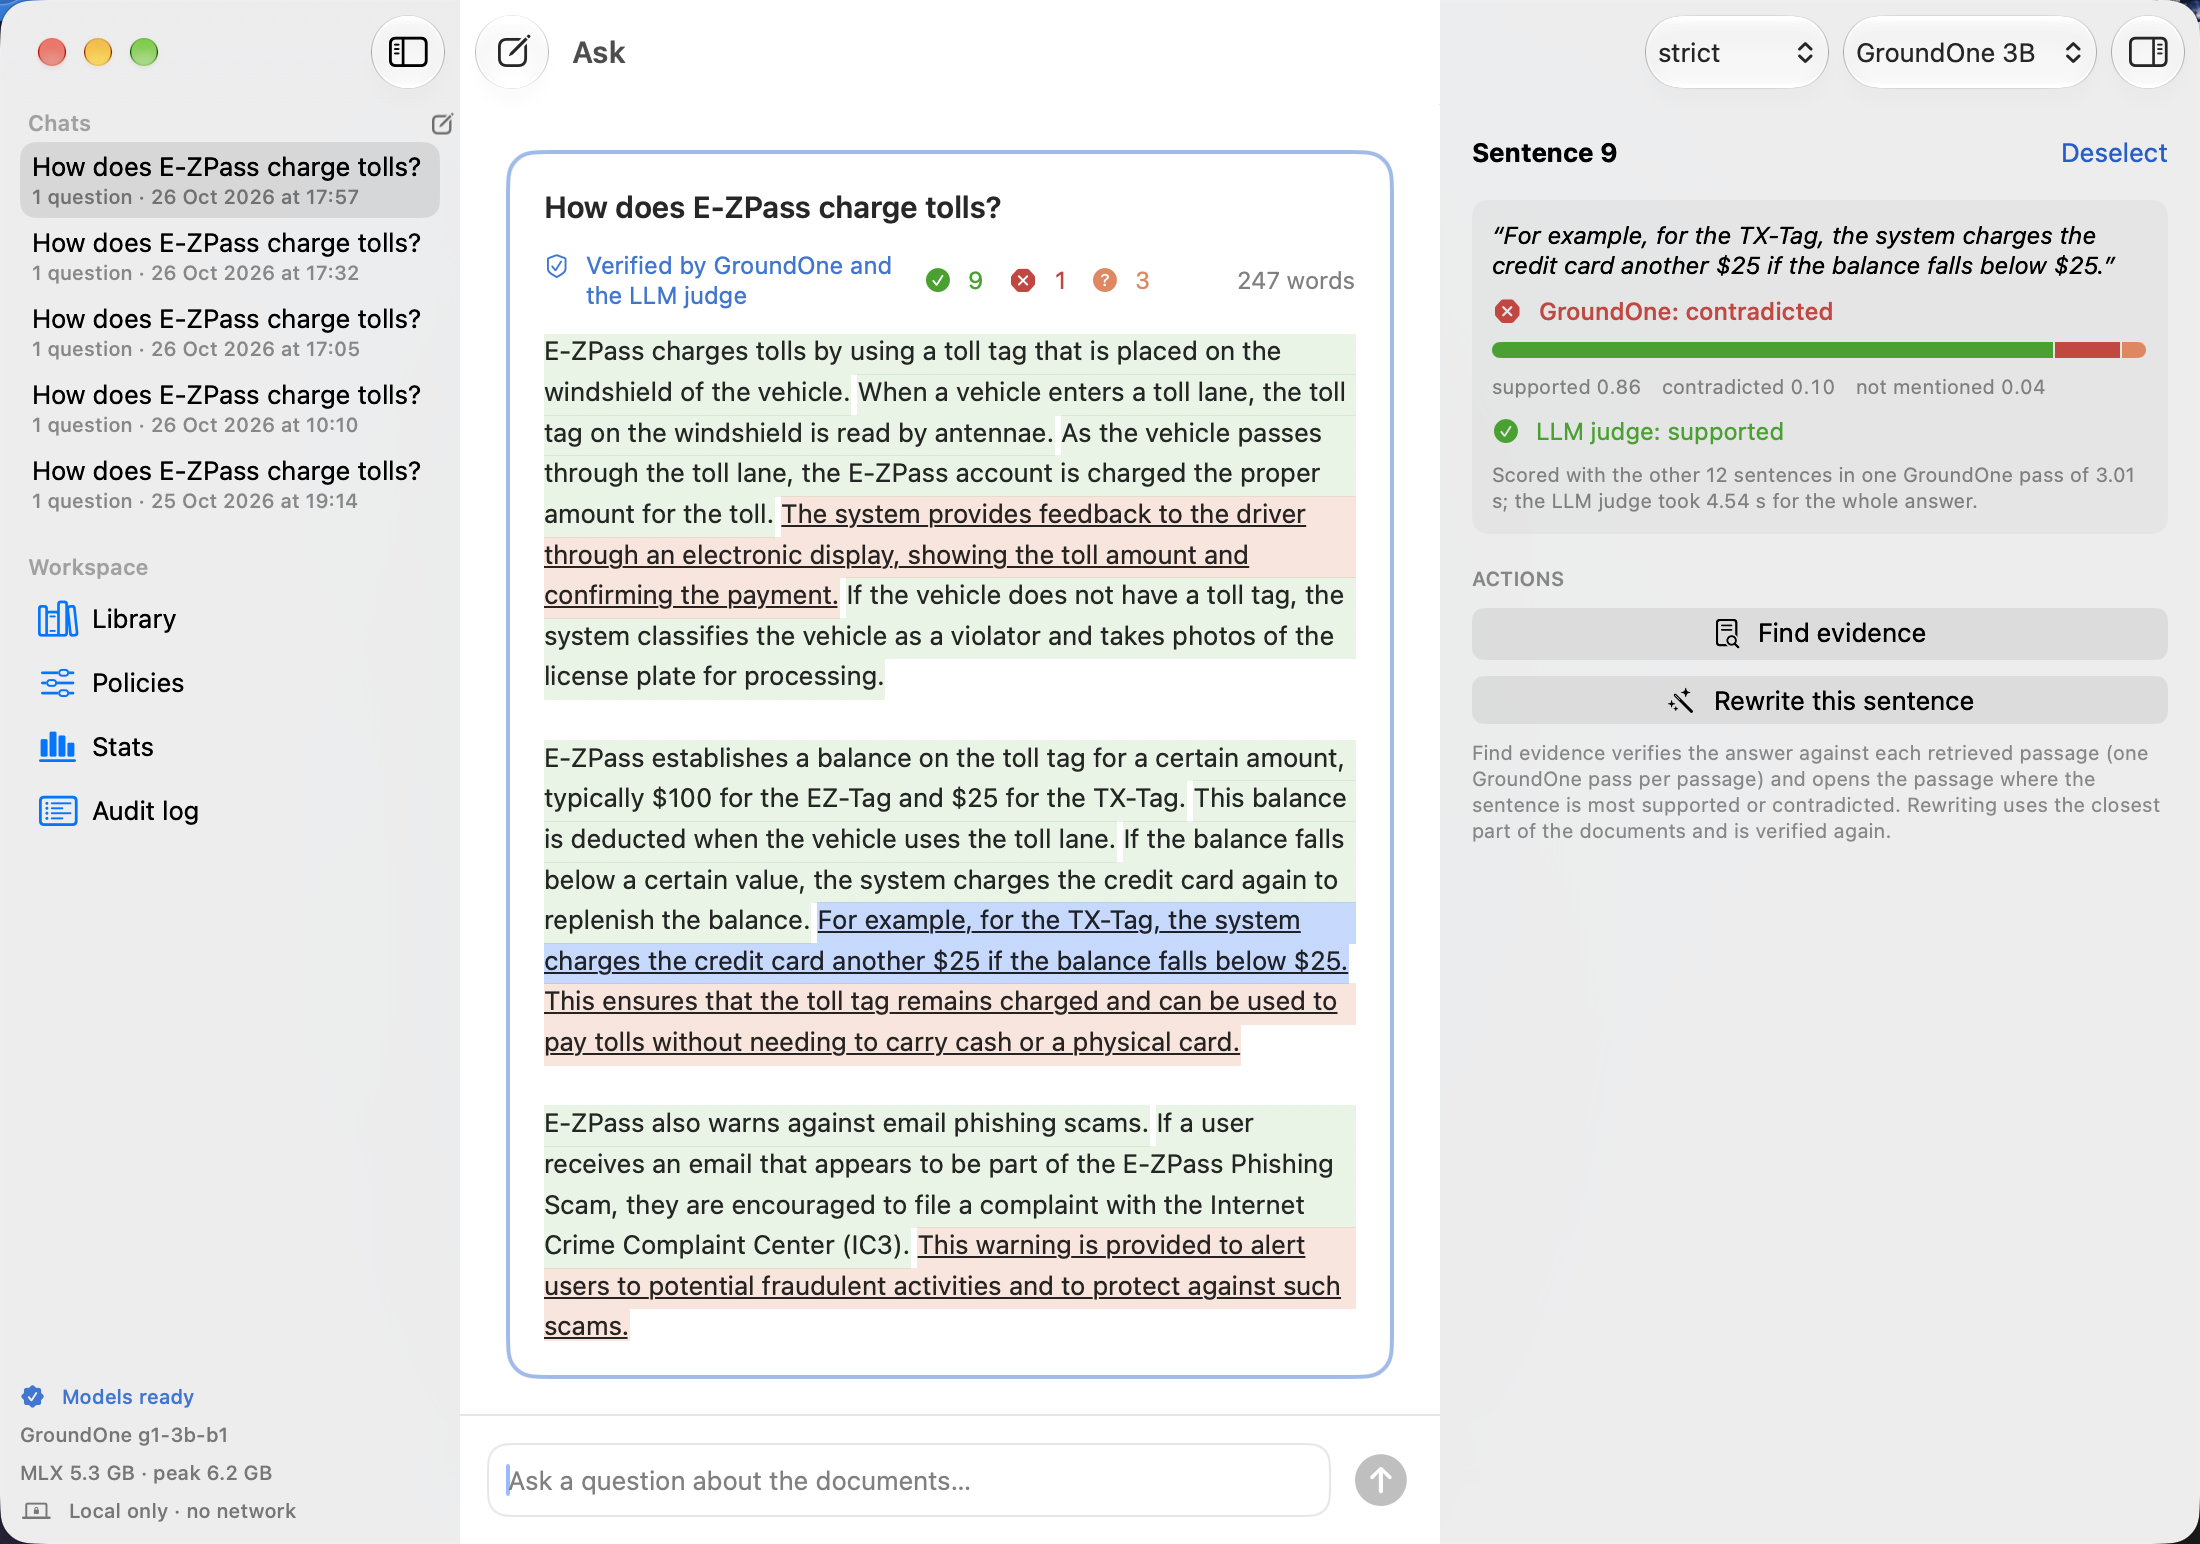
\includegraphics[width=\textwidth]{images/studio/43-sentence.png}
\caption{The panel of a selected sentence: calibrated probabilities of GroundOne, verdict of the LLM judge, times and
available actions.}
\label{fig:studio-sentence}
\end{figure}

\paragraph{Evidence.} GroundOne indicates whether a sentence is supported, but not by which passage
(Section~\ref{sec:disc-limitations}). The application reconstructs this information in two steps. In the first, it
verifies the answer against each retrieved passage separately, with one forward pass per passage, and picks the one in
which the sentence obtains the highest probability of support, or of contradiction if the sentence is contradicted. In
the second, within the chosen passage, it locates the sentence closest to the one in the answer, weighting the shared
words by their rarity in the passage. The document preview opens with that span highlighted
(Figure~\ref{fig:studio-evidence}). This is the first prototype of the readout per passage listed among the future
developments (Section~\ref{sec:concl-future}). It has not been evaluated, because RAGTruth does not indicate which
passage supports a sentence, and the application presents it as evidence suggested by GroundOne. The computation runs
only on request and is cached: with six passages it costs six forward passes, that is, a few seconds with the 3B, and it
does not change the times of the main verification.

\begin{figure}[htbp]
\centering
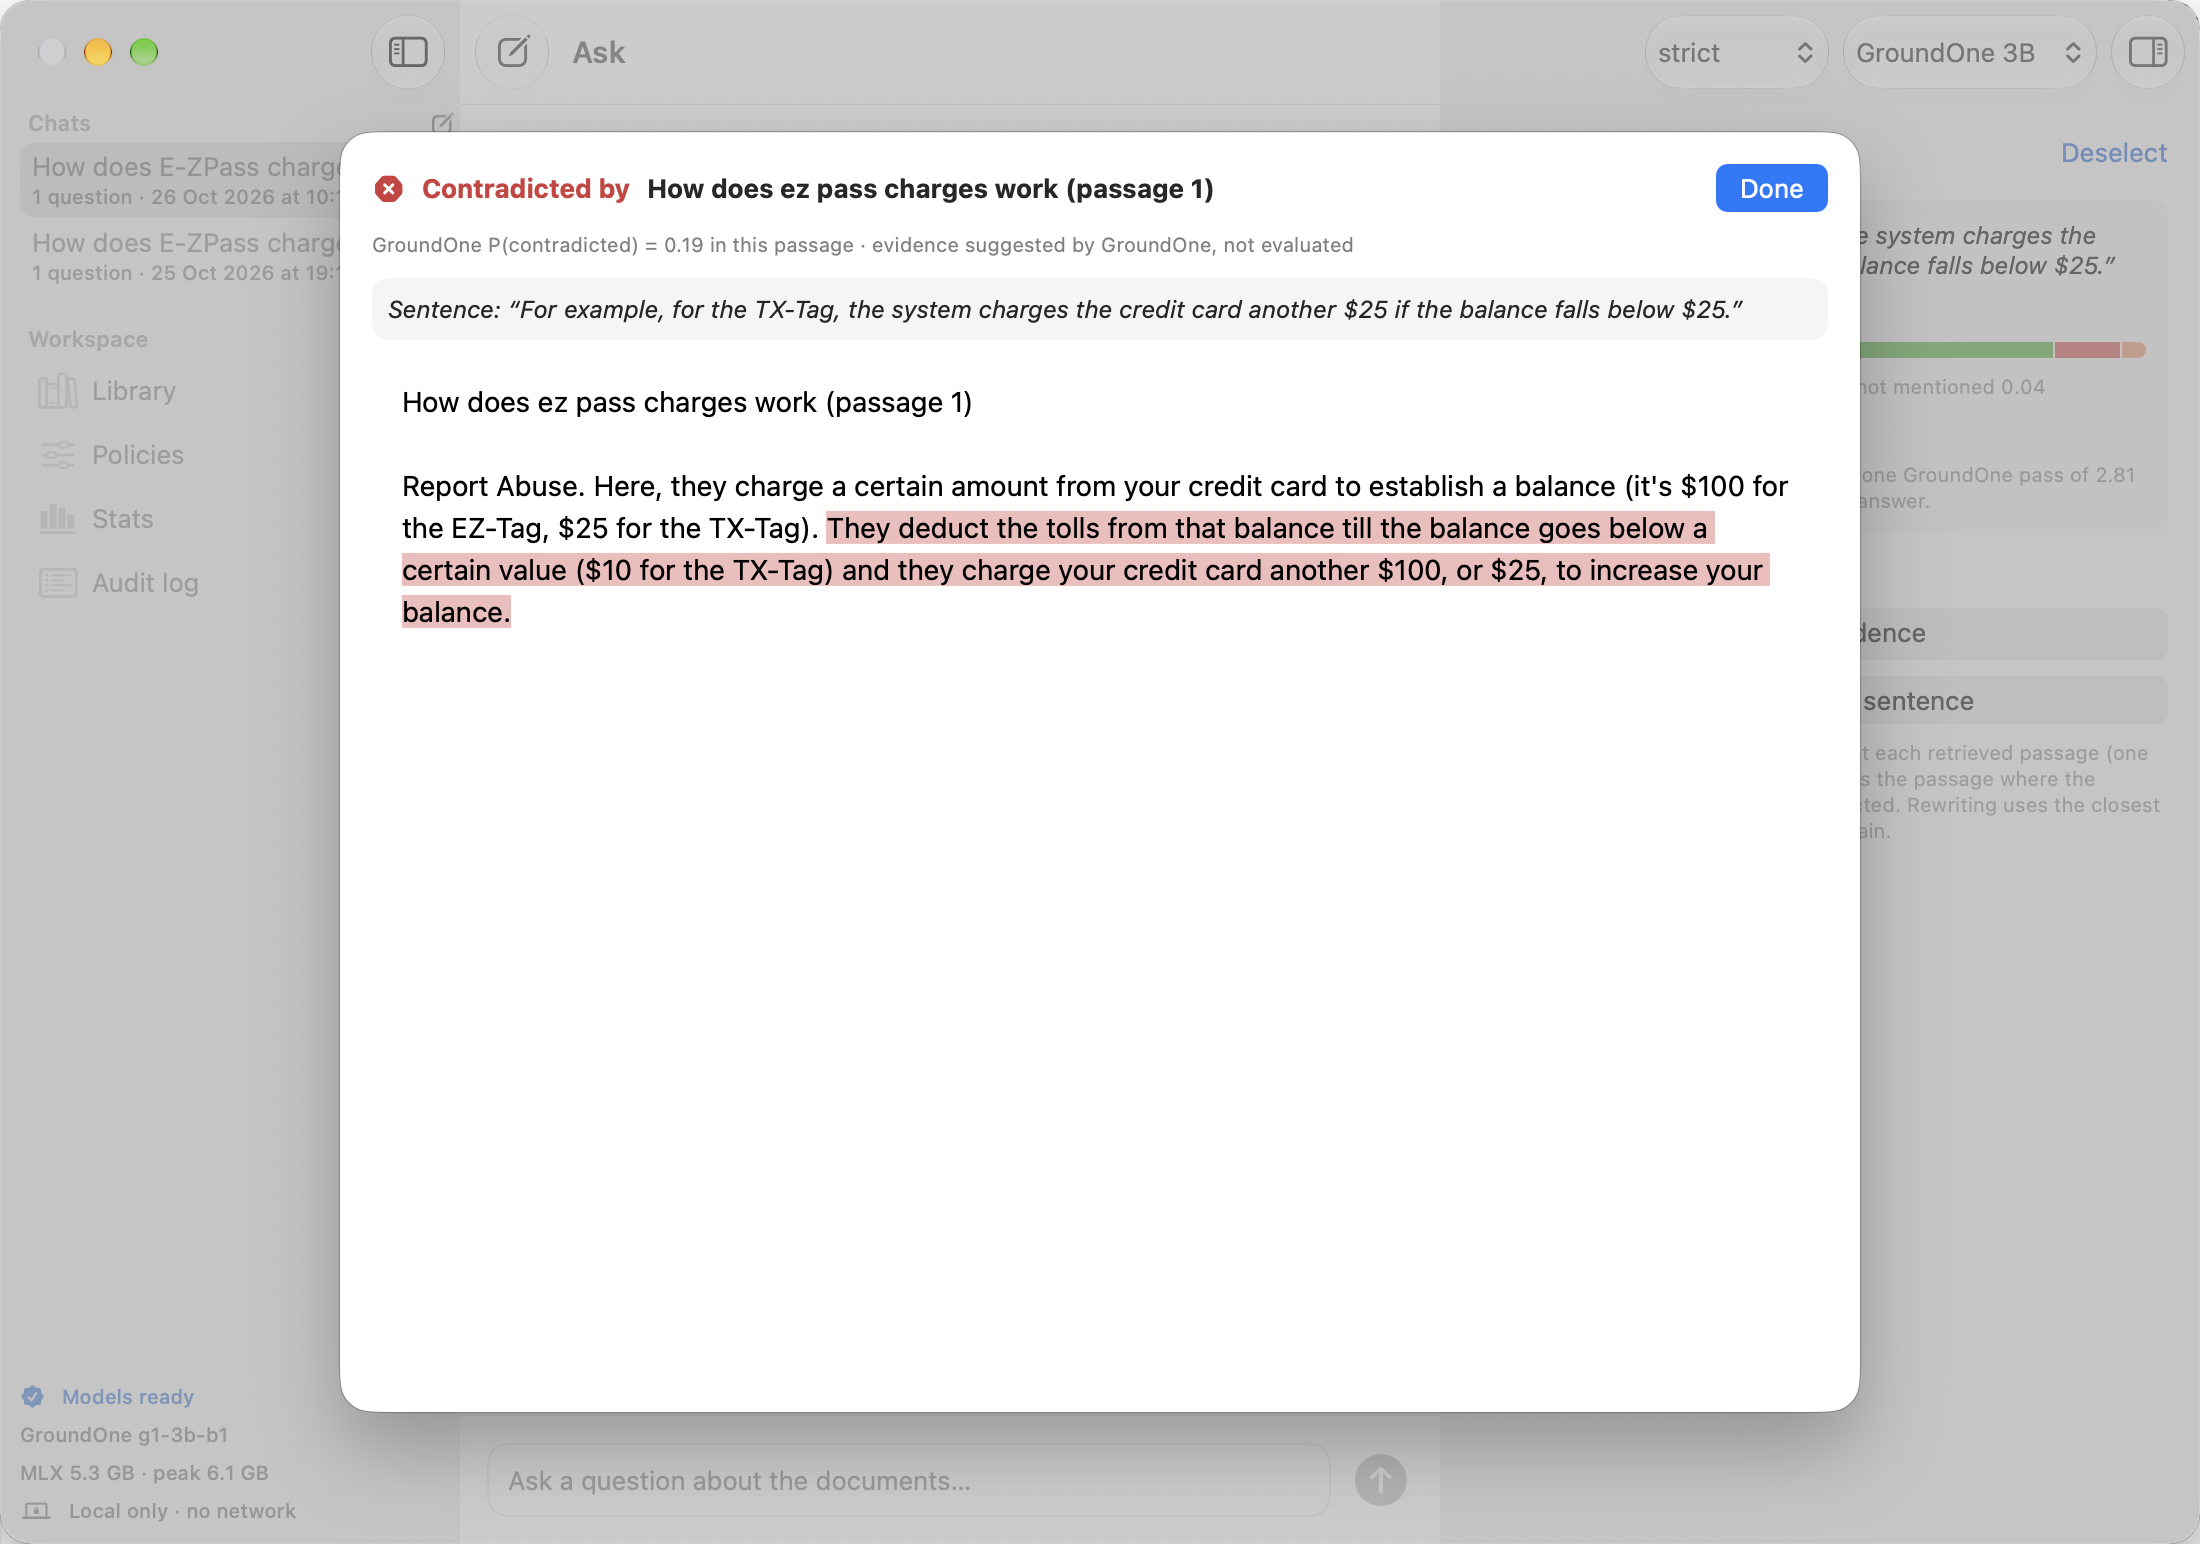
\includegraphics[width=\textwidth]{images/studio/44-evidence.png}
\caption{The evidence for a sentence: the passage that, according to GroundOne, most clearly contradicts the sentence,
with the closest span highlighted.}
\label{fig:studio-evidence}
\end{figure}

\paragraph{Targeted rewriting.} Rewriting follows a principle of the verify-and-revise loops that have proved effective
in the literature: an external critic, or retrieved evidence, flags the errors and the generator changes only what has
been flagged~\cite{gao2023rarr,gou2024critic}, whereas spontaneous self-correction, without an external signal, does not
reliably improve the answers~\cite{huang2024cannotselfcorrect}. GroundOne is the critic, and a cheap one: verifying again costs a single prefill, and not even a full one. The instructions and the sources, already read ahead or at the first verification, stay in the KV cache (Section~\ref{sec:method-readout}), so the new version only requires reading the rewritten answer, which in the measurements of Section~\ref{sec:results-latency-split} makes the verification 3.4 times faster with the 3B. The part of the answer before the first rewritten sentence is also kept, together with the verdicts of its sentences, so the reading restarts at the first change: when the last sentence is rewritten, the verification is about six times faster than with the sources alone (Table~\ref{tab:results-answer-prefix}). The LLM judge, when requested, reuses the cache of the sources, but writes all its verdicts again; the timing panel shows how many tokens were reused. For every sentence to be rewritten, the generator receives a short request, with the
sentence and only the excerpt of the document that concerns it, and an instruction that depends on the type of error. A
contradicted sentence must be corrected with the facts of the source and cannot be deleted: if the generator does not
return a usable sentence, the original one stays in place and is resubmitted in the next round. A sentence that is not
mentioned must be rewritten with what the source says on the same point, or removed if the source does not address it. In both cases the instruction explicitly asks not to return the sentence unchanged. If the generator copies it anyway, which happens with a small model, the request is repeated once, quoting the copy and rejecting it; if the second attempt also returns the same sentence, the sentence stays as it is, flagged, and the panel shows that the generator could not correct it. It is not retried in later rounds, because with greedy decoding the reply would be the same. The other sentences remain unchanged. The maximum number of rounds and the classes to be corrected are set by the
policy.

\paragraph{Policy and threshold.} A policy is a small JSON file that specifies which verdicts are to be corrected, how
many rewriting rounds are allowed, what to do if the error persists (highlight, hide the sentence or abstain) and which
threshold to use: the one fitted on the dev set or one chosen by the user. The two default policies correspond to the
two readings already introduced in the thesis (Section~\ref{sec:method-calibration}): the strict policy corrects both
contradicted and not-mentioned sentences, the lenient policy only the former.

\paragraph{Conversations and statistics.} Questions are organised into separate conversations, which can be renamed,
deleted and resumed at any time. A dedicated section collects the statistics of all the verifications run in the
application, including those of previous sessions (Figure~\ref{fig:studio-stats}): the time of GroundOne and that of the
LLM judge as a function of the number of sentences, the agreement between the two on the same sentences, the distribution of
the verdicts and the cost the same verification would have had with a cloud LLM judge. The cost uses the same list prices
as Table~\ref{tab:disc-cost}: the input tokens are those of the document and the answer plus the instruction; the output
tokens are those actually written by the local LLM judge or, if the LLM judge was not run, their mean number per sentence
measured in the thesis. The cost of the electricity consumed locally, estimated from the verification time and from the
power measured in Section~\ref{sec:results-energy}, is subtracted from it.

\begin{figure}[htbp]
\centering
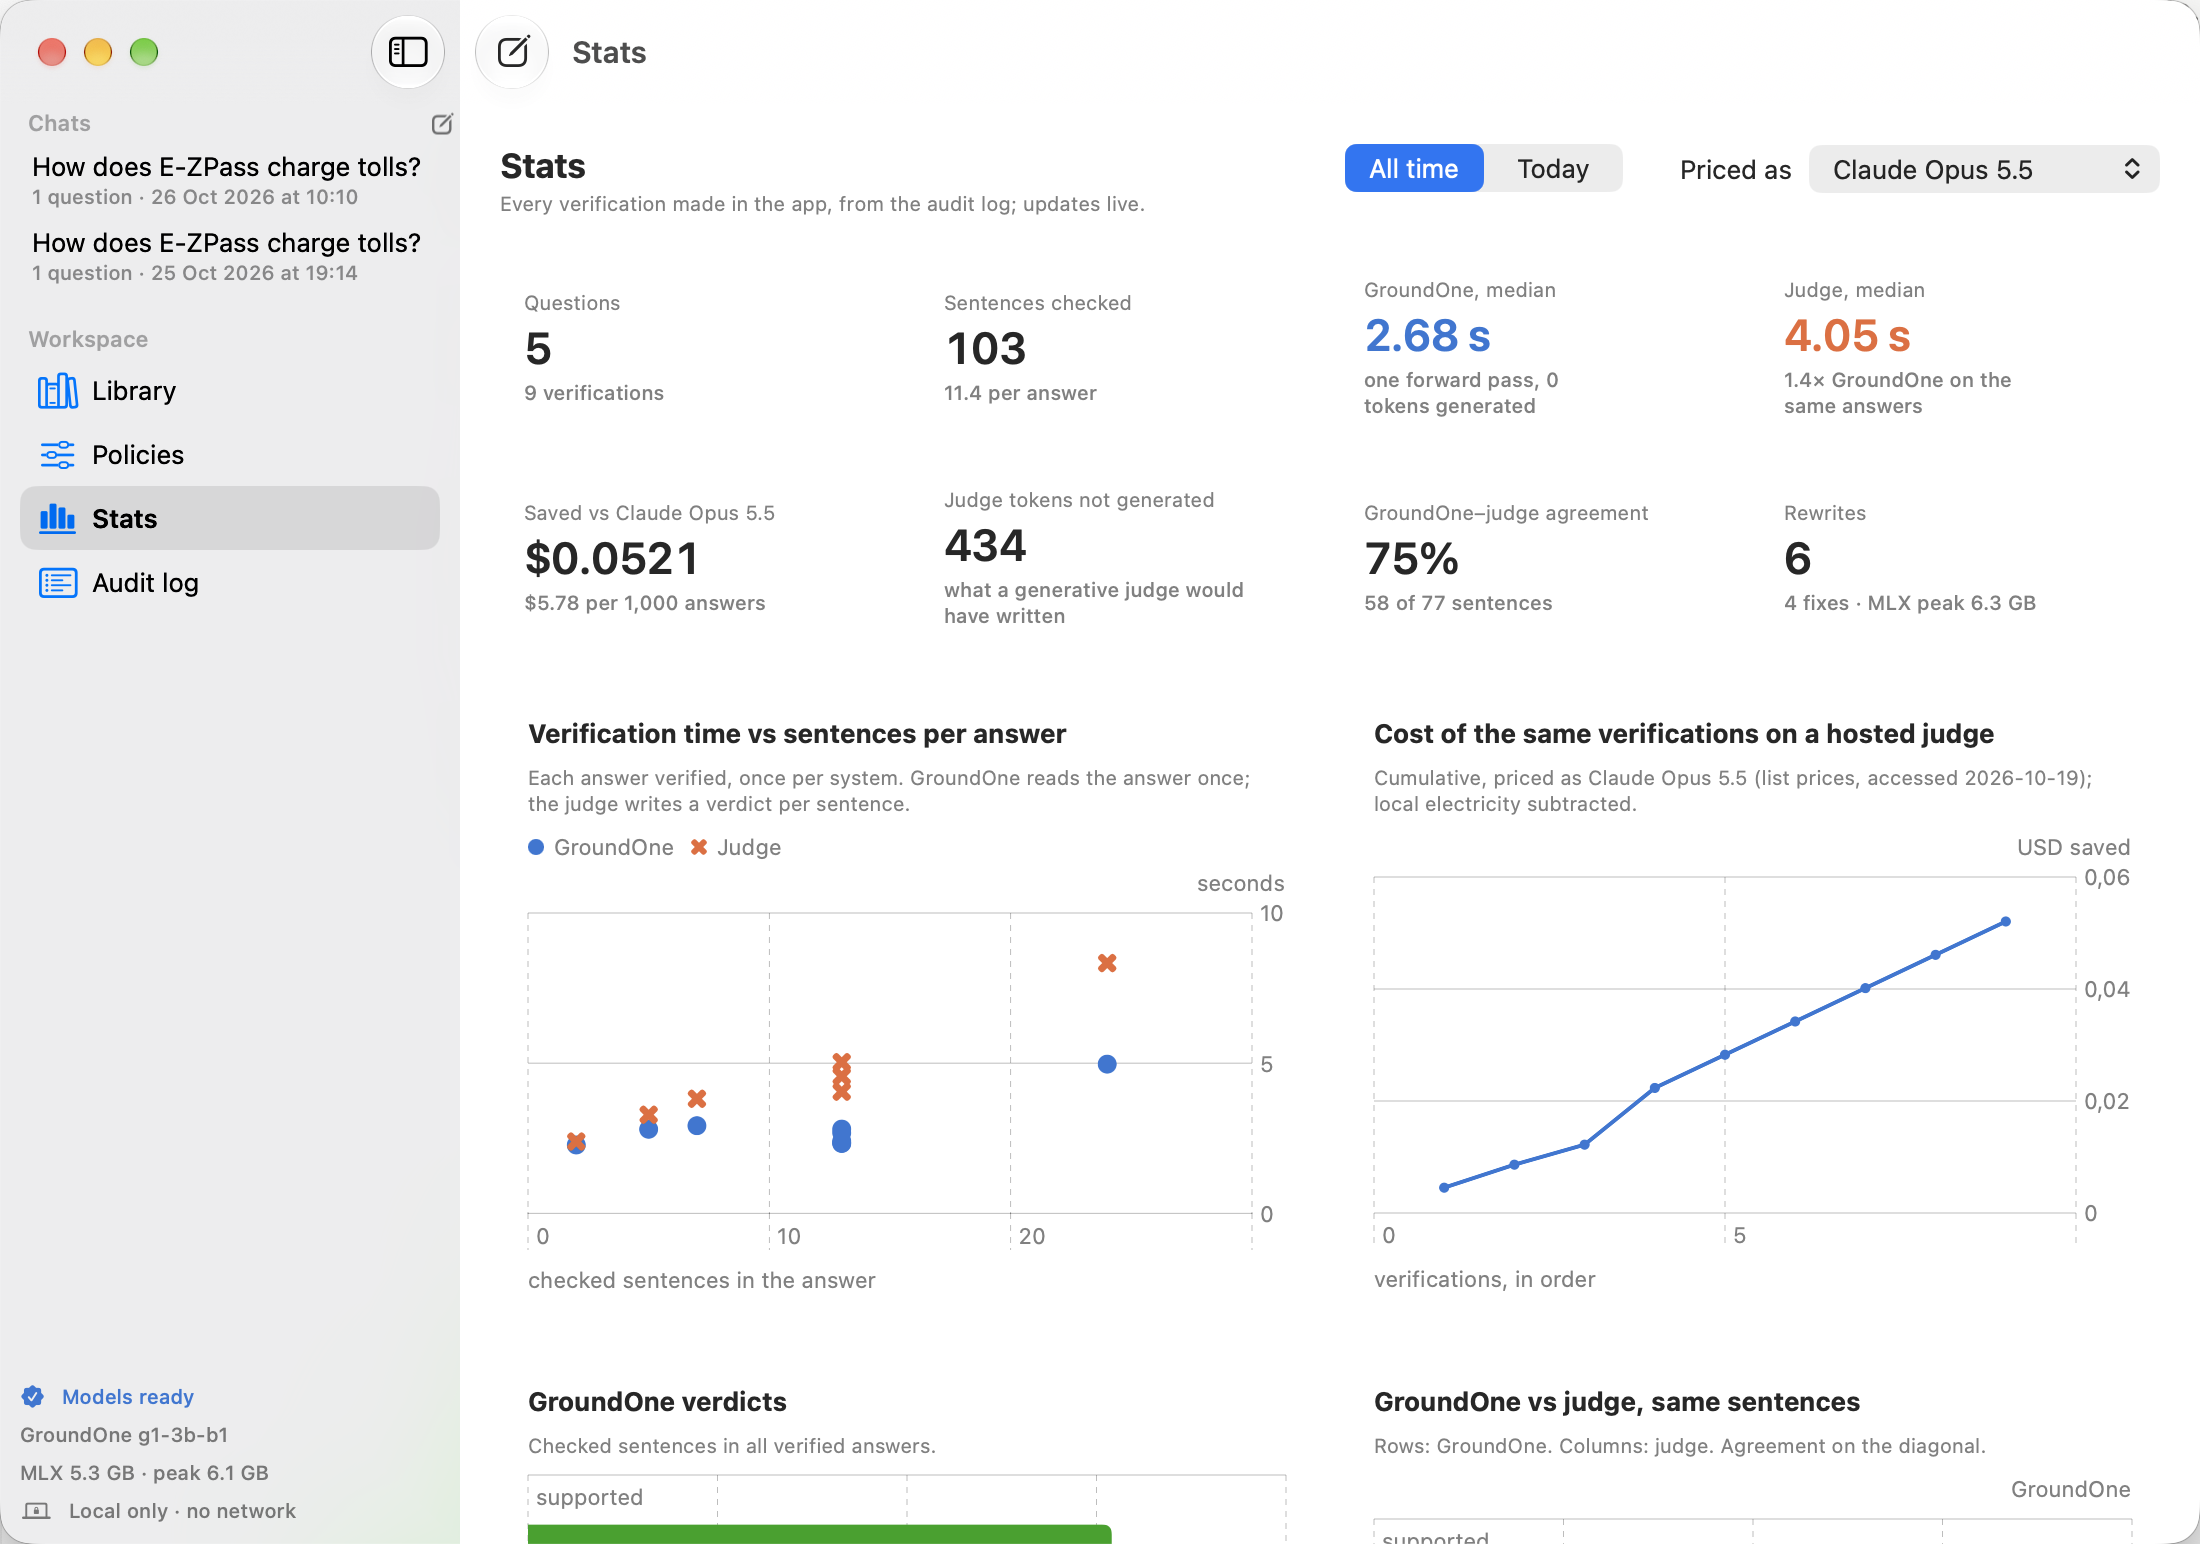
\includegraphics[width=\textwidth]{images/studio/46-stats.png}
\caption{The statistics section: key indicators, verification time as a function of the number of sentences for
GroundOne and for the LLM judge, and cost of the same verification with a cloud LLM judge.}
\label{fig:studio-stats}
\end{figure}

\paragraph{Persistence.} All the data of the application reside on the local disk, in the application support folder
provided by macOS, without any database server (Table~\ref{tab:studio-persistence}). The support folder was preferred to
the user's document folders for a practical reason: macOS protects the Desktop and Documents folders and makes access to
them conditional on an explicit permission, which an application would have to request at launch.

\begin{table}[htbp]
\centering
\caption{Data persistence in the application. Everything resides on the local disk.}
\label{tab:studio-persistence}
\small
\begin{tabular}{>{\raggedright\arraybackslash}p{3.6cm}>{\raggedright\arraybackslash}p{3.4cm}>{\raggedright\arraybackslash}p{6.0cm}}
\toprule
Data & Format & Use \\
\midrule
Conversations & One JSON file per conversation. & Questions, answer versions, verdicts, times; resumption of conversations. \\ \addlinespace[2pt]
Action log & Append-only JSONL file. & One line for every generation, verification and rewriting; basis of the statistics and of the browsable log. \\ \addlinespace[2pt]
Library & SQLite database. & Full-text index for BM25 and passage embeddings, with the origin of each passage. \\ \addlinespace[2pt]
Policies & JSON files. & Selectable decision and rewriting rules. \\ \addlinespace[2pt]
KV cache of the sources & In memory only. & Instructions, the last documents already read (also ahead, while the user reads the answer) and the last answer verified, reused by later verifications; not saved to disk. \\
\bottomrule
\end{tabular}
\end{table}

\section{Case study: injected errors}
\label{sec:studio-casestudy}

Answers generated for free questions have no reference label: measuring on them how much the verify-and-rewrite loop
improves the answer would require an independent judgement on every rewritten sentence. The case study therefore uses
injected errors, whose position is known in advance and does not depend on GroundOne.

\paragraph{Protocol.} From the T1 answers whose reference labels are all ``supported'' and which GroundOne 3B accepts in
full, 100 were drawn from the three tasks: 46 from summarisation, 29 from question answering and 25 from data-to-text. A
single error was injected into each, of four types, 25 per type: a number replaced with a value absent from the
document, a name replaced with an invented one, a shifted date, or an invented sentence inserted after an existing one.
The answers then go through the same engine as the application: GroundOne verifies the answer, the LLM judge verifies it in
turn for the comparison, and the strict policy rewrites the flagged sentences for up to two rounds. An error counts as
removed when the wrong value no longer appears in the text, or when no sentence remains similar to the invented one. The
case study does not use retrieval: the document is that of T1.

\begin{table}[htbp]
\centering
\caption{Case study on injected errors: 100 answers of T1, one error each, GroundOne 3B and the 4-bit
Qwen2.5-3B-Instruct generator in the same process, without the embedding model, with the KV cache of the sources active. Detection is computed on the 98 answers
in which the sentence with the error receives its own verdict.}
\label{tab:studio-casestudy}
\small
\begin{tabular}{>{\raggedright\arraybackslash}p{9.4cm}c}
\toprule
Measure & Value \\
\midrule
Sentence with the error flagged by GroundOne & 97 of 98 \\
Sentence with the error flagged by the LLM judge & 84 of 98 \\
False alarms of GroundOne on the other sentences & 1.8\,\% \\
Answers still containing the error: without the loop, after one and after two rounds & 100\,\%, 8\,\%, 6\,\% \\
Errors removed by restoring the value of the source & 42 \\
Errors removed by rewriting the sentence & 1 \\
Errors removed by deleting the sentence & 51 \\
Remaining errors: still flagged / never flagged & 3 / 3 \\ 
Sentences the generator copies even at the second attempt & 3 \\
Other sentences left identical & 98.0\,\% \\
Answers accepted by GroundOne at the end & 94\,\% \\
Median time per answer: GroundOne, LLM judge, rewriting per round & 1.74\,s, 2.36\,s, 0.92\,s \\
Memory allocated by MLX: after loading and at peak & 5.1\,GB, 6.7\,GB \\
\bottomrule
\end{tabular}
\end{table}

\paragraph{Results.} Table~\ref{tab:studio-casestudy} and Figure~\ref{fig:studio-outcomes} summarise the case study. In
98 answers the sentence with the error receives its own verdict; in the other two, the segmenter merges it with an
introductory sentence without checkable content, and the sentence is not scored. GroundOne flags the error in 97 of the
98 answers, the LLM judge in 84. The loop reduces the answers that still contain the error from 100\,\% to 8\,\% after one round and to 6\,\% after two, according to the automatic count. The way in which errors are removed matters as much as
their number. For replaced numbers and dates, in most cases the generator restores the value of the source: 19 numbers and 16 dates out of 25. Invented sentences, instead, are deleted, all 25 of them, which is the appropriate correction.
Invented names, finally, are correctly labelled as not mentioned, and for this reason they are mostly removed, 18 out of
25, rather than replaced with the original one, 7 out of 25: the sentence loses the error, but also the information. The copy check intervenes three times: in three sentences the generator returns the same sentence even at the second attempt, and the sentence stays flagged. Of the six answers that keep the error, three remain flagged and are therefore highlighted by the policy. In the other three
the error is never flagged: in one, the probability of support, 0.93, is just above the threshold of 0.925; in the other
two, the injected sentence does not receive its own verdict.

\begin{figure}[htbp]
\centering
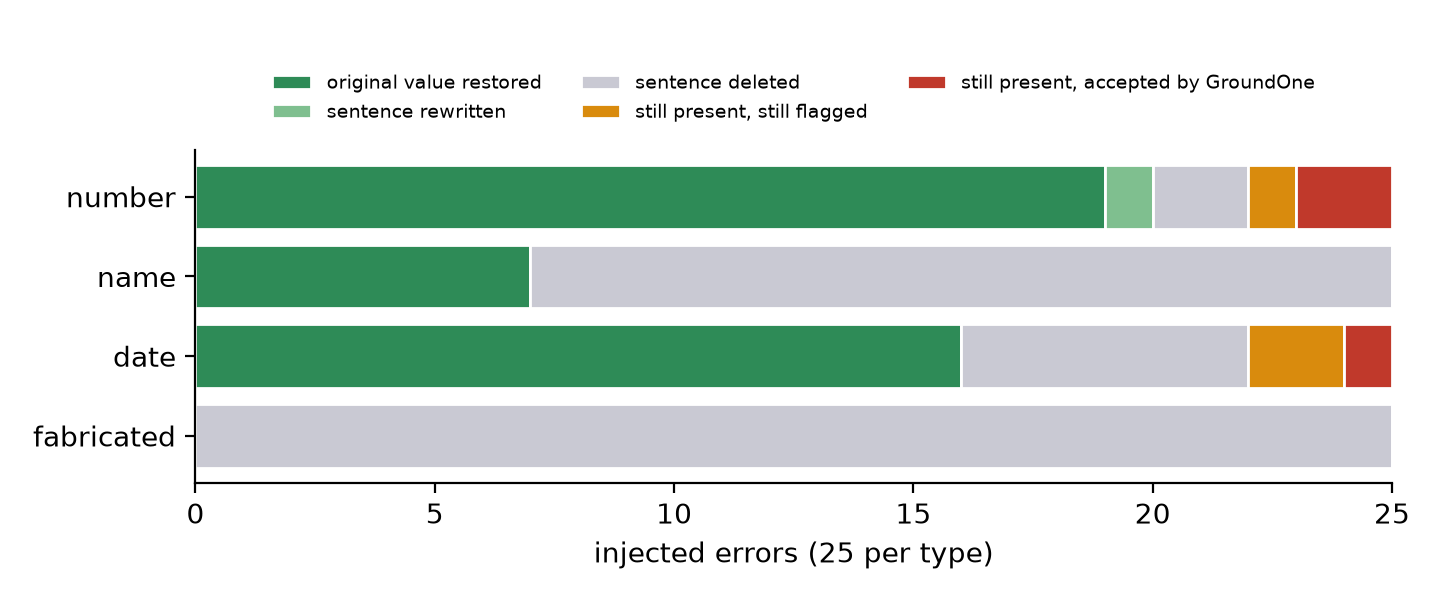
\includegraphics[width=\textwidth]{images/studio/casestudy_outcomes_g1-3b-b1-set2-final.png}
\caption{Outcome of each injected error after the loop, by error type, with GroundOne 3B: value restored from the
source, sentence rewritten, sentence deleted, error still present and flagged, error accepted by GroundOne.}
\label{fig:studio-outcomes}
\end{figure}

\paragraph{The type of error decides the repair.} Repeating the case study with GroundOne 0.5B as the verifier shows why
the three-class verdict matters, and not only the flag. The 0.5B flags the error in 97 answers out of 98, like the 3B,
but labels almost all the replaced numbers and dates as not mentioned (44 out of 50), whereas the 3B recognises them as
contradicted (40 out of 50). For a sentence that is not mentioned, rewriting may remove the sentence, and the generator
does so: with the 0.5B, 84 errors are removed by deleting the sentence and only 12 by restoring the value. The answers
that keep the error fall to 3\,\%, but at the price of lost information and of many false alarms: the 0.5B flags
17\,\% of the other sentences, which are correct, and only 84\,\% of them remain unchanged. The distinction between a
contradicted and a not-mentioned sentence, which Chapter~\ref{sec:method} motivates in the abstract, here decides
whether the correction restores the information or eliminates it.

\paragraph{Times.} The comparison of times confirms the picture of Section~\ref{sec:results-latency}. On these answers,
with a median of about 770 tokens between document and answer and of six scored sentences, the median time of the LLM judge is 1.36 times that of GroundOne (2.36 against 1.74 seconds, both reading the sources for the first time), and the LLM judge writes around twenty tokens, whereas GroundOne generates none. The
difference is small because the terse LLM judge writes little and the answers are short. The comparison on detection, 97
errors flagged against 84, instead favours GroundOne by construction: the answers were chosen among those that GroundOne
accepts in full, a filter that the LLM judge did not pass, and the false alarms of the LLM judge on the correct sentences were
not measured.

\paragraph{A comparison at equal compute.} On 60 new T1 answers, generated by the model for each task, the complete
loop, that is, answer, verification and up to two rounds of targeted rewriting, was compared with a strategy that
corrects nothing: generating up to three answers with sampling and keeping the first one that GroundOne accepts. The
first answer is accepted in 52\,\% of the cases. At the end, the loop brings the accepted answers to 70\,\%, multiple generation to 62\,\% (42 and 37 answers out of 60, a small difference on this sample). The loop, however, generates half the tokens, 115 against 218 at the median, in a similar time, 6.3 seconds against 7.0: multiple generation also verifies every sample on the same document, and therefore reuses its KV cache. Rewriting only the flagged sentences thus gets at least as many answers accepted as regenerating them from scratch, with half the generation. Part of the answers remains flagged because the 3B generator
fails to correct a contradicted sentence, which the loop cannot delete.

\paragraph{A larger generator.} The generator can be chosen in the application: besides the 3B,
Qwen2.5-7B-Instruct at 4 bits is available. On the same case study the 7B corrects every error that GroundOne flags: the
answers that still contain the error fall to 3\,\%, that is, to the three in which GroundOne does not flag it, against
6\,\% with the 3B, and those accepted by GroundOne rise to 98\,\%. The price is time and memory: a rewrite costs 2.1
seconds per round against 0.9, and the peak of memory allocated by MLX rises to 9.2\,GB against 6.7. On the twelve
example questions of the library, moreover, the 7B writes answers of similar length (276 words at the median against
250) in more than twice the time (17.7 seconds against 7.6), and adds more content that the sources do not report:
GroundOne considers 66\,\% of its sentences supported, against 85\,\% of those of the 3B. For this reason the 3B remains
the default generator.

\paragraph{How to read the results.} Three caveats delimit the scope of the case study. The first concerns detection.
The answers were chosen among those that GroundOne accepts, and the injected errors are clear-cut: values and names
absent from the document. The high share of flagged errors therefore shows how the loop works, not the recall of
GroundOne, which is measured in Chapter~\ref{sec:results}. The second concerns the rewritten sentences: they have no
reference label, and their correctness is judged only by GroundOne, the same model that decides when to stop the loop. A
rewriting that falls into a blind spot of the model is therefore counted as successful, and the automatic count records
only the disappearance of the injected error, not any new errors introduced by the rewriting. For this reason the
results are expressed as answers ``accepted by GroundOne'', not as correct answers, and the 94\,\% of accepted answers includes three answers that still contain the error. The third concerns the generator. A 3B model sometimes cannot
correct a sentence and sometimes removes it: 26 of the 51 errors removed by deletion also take away correct information,
so part of the accepted answers is simply shorter.

\section{An example: a subtle numerical error}
\label{sec:studio-example}

The question of Figure~\ref{fig:studio-native} shows in miniature both the value and the limits of the system. Among the
thirteen sentences of the answer, the generator writes that, for the TX-Tag card, the credit card is topped up by 25
dollars when the balance falls below 25 dollars. The retrieved passage instead says that the top-up happens when the
balance falls below 10 dollars. The sentence follows the source almost word for word, and it is precisely the type of
error that Section~\ref{sec:results-errors} identifies as the hardest for GroundOne. GroundOne assigns it a probability
of support of 0.86, below the threshold of 0.925, and indicates contradiction as the most likely error; the generative
LLM judge considers it supported. GroundOne also flags as not mentioned three sentences that add details or inferences
absent from the documents, for example that the display shows the toll amount, whereas the LLM judge accepts them all.
Rewriting, however, fails: the 3B generator returns the same sentence, with the same wrong amount, even at the second attempt, which quotes the copy and rejects it. The application detects this and leaves the sentence flagged: the quality of the loop also depends on the generator.

\section{Calibrated probabilities and decision threshold}
\label{sec:studio-threshold}

The example helps to clarify a point that using the application makes evident. The probabilities of GroundOne are
calibrated: on T1, among the sentences to which the 3B assigns a probability of support between 0.80 and 0.925,
93\,\% are actually supported. Yet all these sentences are flagged, because the threshold is 0.925. The two facts are not
in contradiction. Calibration concerns the meaning of the probabilities; the threshold is a decision rule, chosen on the
dev set to maximise the three-way balanced accuracy (Section~\ref{sec:method-calibration}). Since the great majority of
sentences are supported, about 88\,\% in the dev set and 91\,\% in T1, a metric that weighs the three classes equally
pushes the threshold upwards: to find the rare errors, it accepts many false alarms
(Table~\ref{tab:studio-threshold}).

\begin{table}[htbp]
\centering
\caption{Effect of the threshold on the T1 sentences with GroundOne 3B: share of flagged sentences and recall per class.}
\label{tab:studio-threshold}
\small
\begin{tabular}{cccccc}
\toprule
$\tau$ & \makecell{Flagged\\sentences} & \makecell{Recall\\supported} & \makecell{Recall\\contradicted} & \makecell{Recall\\not mentioned} & \makecell{Balanced\\accuracy} \\
\midrule
0.5 & 7\,\% & 0.98 & 0.56 & 0.60 & 0.71 \\
0.8 & 15\,\% & 0.92 & 0.71 & 0.83 & 0.82 \\
0.925 & 25\,\% & 0.82 & 0.78 & 0.89 & 0.83 \\
\bottomrule
\end{tabular}
\end{table}

Moving from 0.8 to 0.925 adds only 0.01 of balanced accuracy, but raises the flagged sentences from 15\,\% to 25\,\%,
when the true errors in T1 are 9\,\%. On the other hand, the error on the TX-Tag card lies precisely in this band: with a
threshold of 0.8 it would have gone unnoticed. The case study offers the mirror example: the only error that GroundOne
lets through has a probability of support of 0.93, just above the threshold. Neither choice is wrong. A high threshold
is preferable when an unflagged error is costly, a lower one when false alarms disturb the user. This is the practical
advantage of calibrated probabilities: the threshold can be chosen knowingly, and the application exposes it as a
parameter of the policy. The label shown for a sentence below the threshold should be read accordingly: it indicates the
most likely type of error, not a certainty, which is why the panel always reports the three probabilities.

\section{Limitations}
\label{sec:studio-limits}

\paragraph{The generator.} The 3B generator writes answers shorter than requested, between about 120 and 250 words
against the 300--500 indicated in the prompt, and does not always manage to correct a flagged sentence: in the example
of Section~\ref{sec:studio-example} it returns the sentence unchanged. A larger generator, for example a 4-bit 7B, would
still fit in the memory of the laptop and should improve both aspects, but it has not been evaluated.

\paragraph{The rewritten sentences.} The correctness of the rewritten sentences is judged only by GroundOne. An
independent check, with a second verifier such as a specialised encoder or with a human reading of a sample, would make
it possible to measure how many accepted rewritings are actually correct.

\paragraph{The evidence.} The suggested evidence has not been evaluated, because the data do not indicate which passage
supports each sentence. It is a demonstration feature.

\paragraph{Scope.} The application inherits the limits of GroundOne (Section~\ref{sec:disc-limitations}): it verifies
documents and answers in English, in the domain of the training data, and it relies on the retrieved documents, not on
the truth of the world. Questions that concern the whole library, for example an overview of the documents, are beyond
the reach of a system that retrieves six passages. The interface, finally, runs only on macOS, and the 3B generator and
verifier are subject to the Qwen research licence (Section~\ref{sec:setup-licences}): the application is a research
prototype, not a product.
